\documentclass{beamer}

%------------------------------------------------------------
% THEME & STYLING
%------------------------------------------------------------
\usetheme{Madrid}
\usecolortheme{default}
\setbeamertemplate{navigation symbols}{} % Hides navigation symbols

%------------------------------------------------------------
% CUSTOM FOOTER DEFINITION
%------------------------------------------------------------
\setbeamertemplate{footline}{
  \leavevmode%
  \hbox{%
  \begin{beamercolorbox}[wd=\paperwidth,ht=2.25ex,dp=2ex]{author in head/foot}%
    \usebeamerfont{author in head/foot}%
    \hspace*{2ex}%
    \insertdate%
    \hfill%
    \textbf{\insertshorttitle}%
    \hfill%
    \insertframenumber/\inserttotalframenumber%
    \hspace*{2ex}%
  \end{beamercolorbox}}%
  \vskip0pt%
}
\setbeamercolor{author in head/foot}{fg=white, bg=structure.fg}

%------------------------------------------------------------
% TOC STYLING (Bold and less space)
%------------------------------------------------------------
\setbeamerfont{section in toc}{series=\bfseries}
\addtobeamertemplate{table of contents}{\vspace{-0.4cm}}{}

%------------------------------------------------------------
% PACKAGES
%------------------------------------------------------------
\usepackage[utf8]{inputenc}
\usepackage{tikz}
\usepackage{lmodern}
\usetikzlibrary{shapes.geometric, arrows, positioning, fit}

%------------------------------------------------------------
% TIKZ STYLES FOR BLOCK DIAGRAM
%------------------------------------------------------------
\tikzstyle{block} = [rectangle, draw, fill=blue!10, text width=8em, text centered, rounded corners, minimum height=4em]
\tikzstyle{subblock} = [rectangle, draw, fill=yellow!20, text width=7em, text centered, rounded corners, minimum height=3em]
\tikzstyle{cloud} = [ellipse, draw, fill=gray!20, minimum height=4em]
\tikzstyle{line} = [draw, -latex']

%------------------------------------------------------------
% PRESENTATION METADATA
%------------------------------------------------------------
\title[RESTful Data-Integration API]{%
    \texorpdfstring{
        \textbf{RESTful Schema-Aware Data Integration and Transformation API}
    }{
        RESTful Schema-Aware Data Integration and Transformation API
    }
}
\author[Dijith Dinesh and Team]{%
    \texorpdfstring{
        \begin{tabular}{ll} % Defines two left-aligned columns
            \textbf{Dijith Dinesh}\\
            \textbf{Aaron Paul} & \textbf{Athuljith S} \\ \textbf{Peter Joe Menachery} & \textbf{Pranav Manoj}
        \end{tabular}
    }{
        Dijith Dinesh (Lead), Aaron Paul, Athuljith S, Peter Joe Menachery, Pranav Manoj
    }
}
\institute{Department of Computer Science and Engineering \\ Model Engineering College, Thrikkakara, Kochi 682021}
\date{August 07, 2025}


\begin{document}
%------------------------------------------------------------
% SLIDE 1: TITLE PAGE
%------------------------------------------------------------
\begin{frame}
  \titlepage
\end{frame}

%------------------------------------------------------------
% SLIDE 2: TABLE OF CONTENTS
%------------------------------------------------------------
\begin{frame}
  \frametitle{Table of Contents}
  \tableofcontents
\end{frame}

%------------------------------------------------------------
% SLIDE 3: INTRODUCTION
%------------------------------------------------------------
\section{Introduction}
\begin{frame}
  \frametitle{Introduction}
    \begin{itemize}
        \item This project proposes a universal API that is schema-aware to serve as an intelligent data gateway.
        \pause
        \item Modern applications suffer from brittle integrations, where small backend changes cause major client-side failures.
        \pause
        \item Our system aims to solve the core problems of \textbf{tight coupling}, \textbf{data transformation overhead}, and \textbf{insecure data access} through an object-oriented design.
    \end{itemize}
\end{frame}

%------------------------------------------------------------
% SLIDE 4: PROBLEM STATEMENT
%------------------------------------------------------------
\section{Problem Statement}
\begin{frame}
  \frametitle{Problem Statement}
  \begin{itemize}
    \item \textbf{Tight Coupling:} Client applications are directly tied to the database schema. A simple column rename in the database can break multiple applications.
    \pause
    \item \textbf{Developer Inefficiency:} Engineers waste significant time writing repetitive boilerplate code to fetch, parse, and re-format data for different use cases.
    \pause
    \item \textbf{Security Risks:} Direct database exposure or poorly managed APIs create vulnerabilities and make it difficult to enforce consistent access policies.
  \end{itemize}
\end{frame}

%------------------------------------------------------------
% NEW SLIDE 5: OBJECTIVES
%------------------------------------------------------------
\section{Objectives}
\begin{frame}
    \frametitle{Objectives}
    \begin{itemize}
        \item To design a RESTful API that serves as an \textbf{abstraction layer} over a database, decoupling clients from the schema.
        \pause
        \item To build a \textbf{dynamic query engine} that translates simple URL parameters into secure SQL queries.
        \pause
        \item To implement \textbf{on-the-fly data transformation} into multiple formats (JSON, CSV, XML) with dynamic field renaming.
        \pause
        \item To enforce \textbf{role-based access control (RBAC)} using API keys for enhanced security.
        \pause
        \item To demonstrate core \textbf{Object-Oriented Programming principles} like Inheritance, Polymorphism, and Encapsulation.
    \end{itemize}
\end{frame}

%------------------------------------------------------------
% SLIDE 6: PROPOSED SOLUTION (UPDATED)
%------------------------------------------------------------
\section{Proposed Solution}
\begin{frame}
  \frametitle{Proposed Solution}
  \begin{itemize}
    \item \textbf{A Decoupled API Abstraction Layer:}
    \begin{itemize}
        \item A lightweight, RESTful middleware that intelligently translates simple client requests into complex, secure database queries.
    \end{itemize}
    \pause
    \item \textbf{Core Features:}
    \begin{itemize}
        \item \textbf{Dynamic Querying:} Allows filtering and sorting data via simple URL parameters.
        \item \textbf{On-the-Fly Transformation:} Lets clients request data in any format and rename fields as needed.
        \pause
        \item \textbf{Centralized Security:} Manages access through role-based API keys.
        \begin{itemize}
             \item \small We intentionally use only API keys for authentication. This gives developers the freedom to integrate any user authentication system (e.g., OAuth, JWT) on their end, as our API only needs the final, secure key.
        \end{itemize}
    \end{itemize}
  \end{itemize}
\end{frame}

%------------------------------------------------------------
% SLIDE 7: EXISTING SOLUTION LIMITATIONS
%------------------------------------------------------------
\section{Existing Solution Limitations}
\begin{frame}
  \frametitle{Existing Solution Limitations}
    \begin{itemize}
        \item \textbf{Direct Database Access:} Insecure, brittle, and not scalable.
        \pause
        \item \textbf{Backend-as-a-Service (BaaS):} Offers limited transformation flexibility and can lead to vendor lock-in.
        \pause
        \item \textbf{Manual API Development:} High effort, error-prone, and leads to inconsistent, repetitive codebases.
        \pause
        \item \textbf{Enterprise API Gateways:} Powerful but often too complex and expensive for many projects.
    \end{itemize}
\end{frame}

%------------------------------------------------------------
% SLIDE 8: EXAMPLE API CALLS
%------------------------------------------------------------
\section{Example API Calls}
\begin{frame}[fragile]
 \frametitle{Example API Calls}
\begin{block}{Example 1: Complex Query with JSON Output}
 \small
\textbf{Request:}
\url{/data/phones?where=price:gt:50000&sort=price:desc&format=json&replace=id:no}
\vspace{0.2cm} \\
\textbf{Explanation:} Fetches products costing more than 50000, sorted by price, returning the items with the `id` field renamed to `no` in JSON format. \\
\textbf{Actual Data:} id:number,name:string,price:number \\
\textbf{Output:}
        \begin{verbatim}
        [
          { "no": 101, "name": "pixel","price":79999 },
          { "no": 205, "name": "one plus","price":51999 }
        ]
        \end{verbatim}
 \end{block}
\end{frame}

%------------------------------------------------------------
% SLIDE 9: BLOCK DIAGRAM - HIGH-LEVEL ARCHITECTURE
%------------------------------------------------------------
\section{Block Diagram}
\begin{frame}
  \frametitle{Block Diagram: High-Level Architecture}
  \begin{figure}
  \centering
  \resizebox{1.0\textwidth}{!}{
  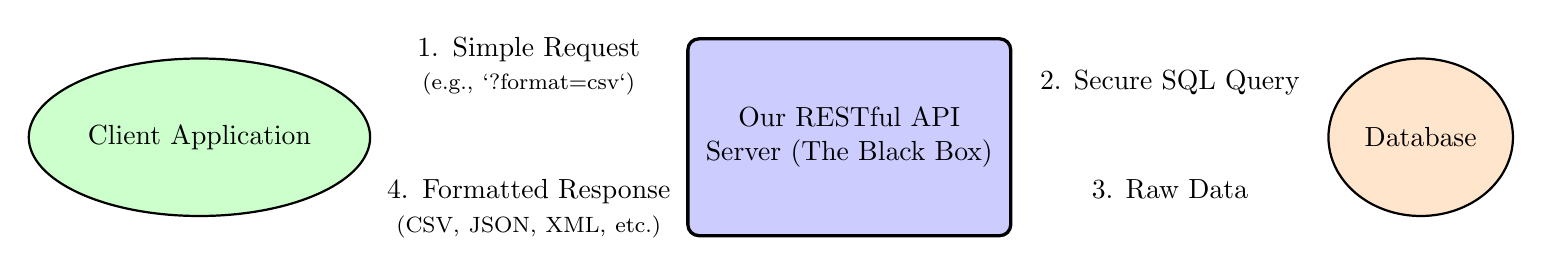
\begin{tikzpicture}[node distance=4cm, auto]
    % Node styles for clarity
    \tikzstyle{actor} = [ellipse, draw, thick, fill=gray!20, minimum size=2cm]
    \tikzstyle{system} = [rectangle, draw, very thick, fill=blue!20, rounded corners, minimum height=2.5cm, text width=11em, text centered]
    \tikzstyle{flowarrow} = [->, very thick]
    
    % Nodes
    \node (client) [actor, fill=green!20] {Client Application};
    \node (api) [system, right=of client] {Our RESTful API Server (The Black Box)};
    \node (db) [actor, right=of api, fill=orange!20] {Database};

    % Arrows with clear, descriptive labels
    \path[flowarrow] (client.east) to [out=20, in=160] node[midway, above, text width=4cm, align=center] {1. Simple Request \\ \footnotesize (e.g., `?format=csv`)} (api.west);
    \path[flowarrow] (api.west) to [out=-160, in=-20] node[midway, below, text width=4cm, align=center] {4. Formatted Response \\ \footnotesize (CSV, JSON, XML, etc.)} (client.east);
    
    \path[flowarrow] (api.east) to [out=20, in=160] node[midway, above] {2. Secure SQL Query} (db.west);
    \path[flowarrow] (db.west) to [out=-160, in=-20] node[midway, below] {3. Raw Data} (api.east);
  \end{tikzpicture}
  }
  \end{figure}
  \vspace{0.5cm}
  \begin{itemize}
      \item Our API acts as an intelligent intermediary, abstracting away database complexity.
  \end{itemize}
\end{frame}

%--------------------------------------------------------------------
% SLIDE 10: BLOCK DIAGRAM - INTERNAL REQUEST FLOW (UPDATED with Auth)
%--------------------------------------------------------------------
\begin{frame}[fragile]
  \frametitle{Block Diagram: Internal Request Flow}
  \begin{figure}
  \centering
  \resizebox{\textwidth}{!}{%
  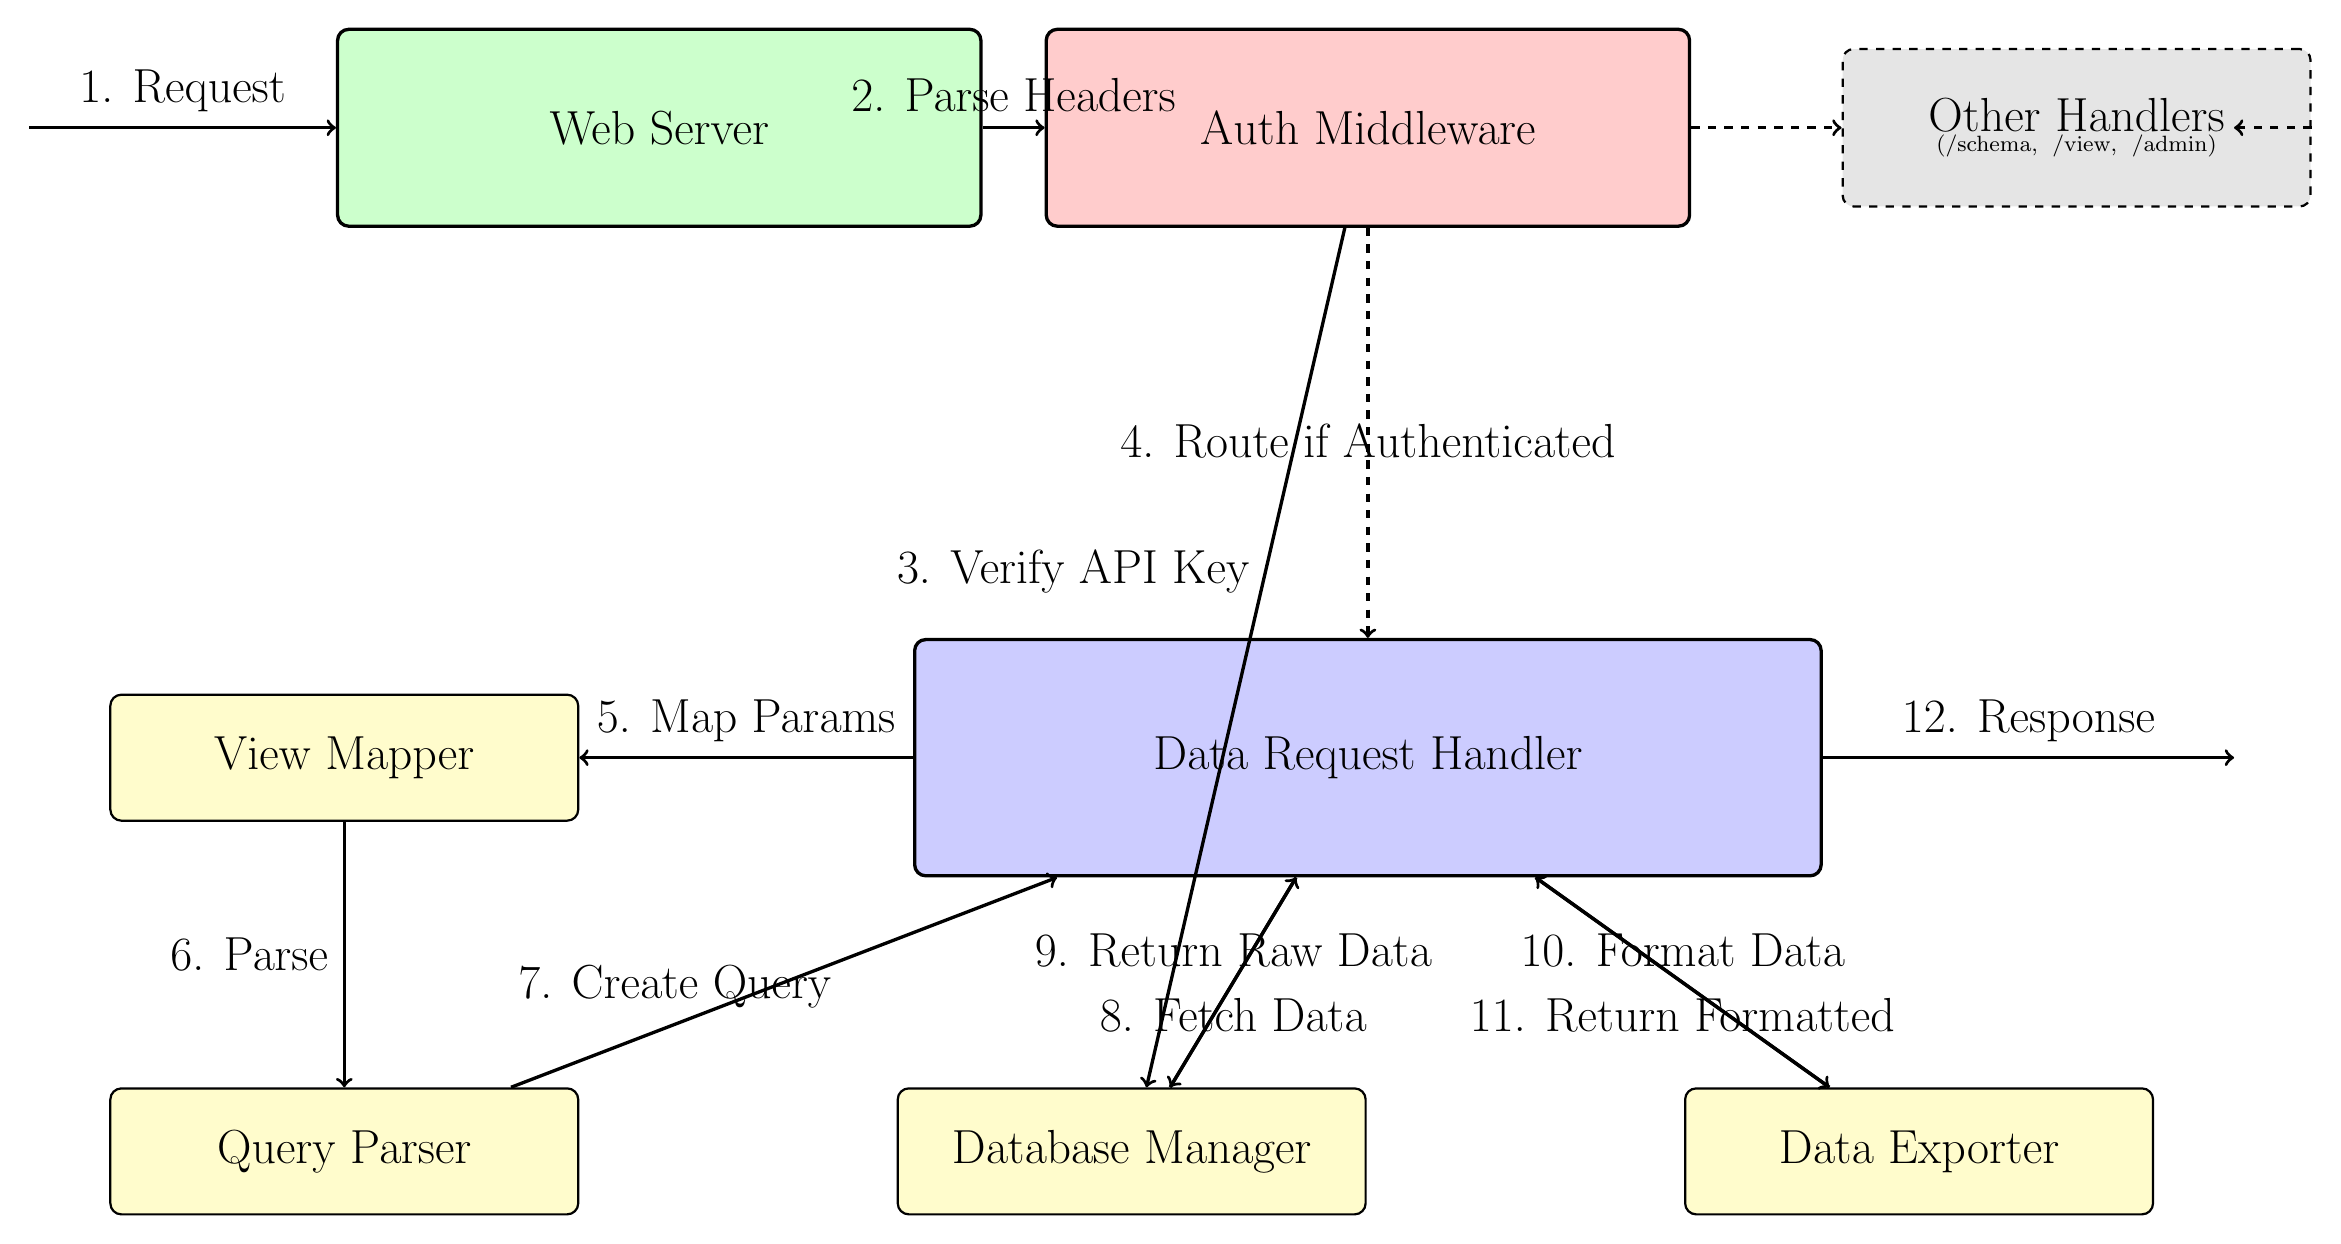
\begin{tikzpicture}
   \fontsize{16pt}{4pt}\selectfont
    % --- STYLES ---
    \tikzstyle{entry} = [rectangle, rounded corners, draw=black, very thick, fill=green!20, text centered, minimum height=2.5cm, text width=14em]
    \tikzstyle{hub} = [rectangle, rounded corners, draw=black, very thick, fill=blue!20, text centered, minimum height=3cm, text width=20em]
    \tikzstyle{spoke} = [rectangle, rounded corners, draw=black, thick, fill=yellow!20, text centered, minimum height=1.6cm, text width=10em]
    \tikzstyle{middleware} = [rectangle, rounded corners, draw=black, very thick, fill=red!20, text centered, minimum height=2.5cm, text width=14em] % New style for middleware
    \tikzstyle{others} = [rectangle, rounded corners, draw=black, thick, fill=gray!20, text centered, minimum height=2cm, text width=10em, dashed]
    \tikzstyle{flow} = [->, very thick]
    
    % --- NODES ---
    % A clean, vertical stack layout for perfect alignment and clarity
    \node (webserver) [entry] at (-6, 8) {Web Server};
    \node (auth)      [middleware] at (3, 8) {Auth Middleware}; % New Auth Middleware node
    \node (handler)   [hub]   at (3, 0) {Data Request Handler};
    
    \node (mapper)    [spoke] at (-10, 0) {View Mapper};
    \node (parser)    [spoke] at (-10, -5) {Query Parser};
    
    \node (dbm)       [spoke] at (0, -5) {Database Manager};
    \node (exporter)  [spoke] at (10, -5) {Data Exporter};
    
    \node (others)    [others] at (12, 8) {Other Handlers \footnotesize (/schema, /view, /admin)};
    
    \coordinate (input) at (-14, 8);
    \coordinate (output) at (14, 0);
    \coordinate (otheroutput) at (14, 8);
    
    % --- ARROWS and LABELS ---
    \draw[flow] (input) -- node[above] {1. Request} (webserver);
    \draw[flow] (webserver) -- node[above] {2. Parse Headers} (auth);

    % Authentication Flow
    \draw[flow] (auth) -- node[left, pos=0.4] {3. Verify API Key} (dbm); % Auth checks DB
    \draw[flow, dashed] (auth) -- node[above, pos=0.6] {4. Route if Authenticated} (handler);

    % Main Data Processing Flow
    \draw[flow] (handler) -- node[above] {5. Map Params} (mapper);
    \draw[flow] (mapper) -- node[left] {6. Parse} (parser);
    \draw[flow] (parser) -- node[above, pos=0.3] {7. Create Query} (handler);
    \draw[flow] (handler) -- node[below] {8. Fetch Data} (dbm);
    \draw[flow] (dbm) -- node[above] {9. Return Raw Data} (handler);
    \draw[flow] (handler) -- node[above] {10. Format Data} (exporter);
    \draw[flow] (exporter) -- node[below] {11. Return Formatted} (handler);
    \draw[flow] (handler) -- node[above] {12. Response} (output);
    
    % Secondary Path to Other Handlers
    \draw[flow, dashed] (auth) -- (others);
    \draw[flow,dashed] (others) -- (otheroutput);

  \end{tikzpicture}%
  }
  \end{figure}
\end{frame}

%------------------------------------------------------------
% SLIDE 11: TECHNOLOGY STACK (UPDATED)
%------------------------------------------------------------
\section{Technology Stack}
\begin{frame}
    \frametitle{Technology Stack}
    \begin{itemize}
        \item \textbf{Programming Language:}
        \begin{itemize}
            \item Java (JDK 11+)
        \end{itemize}
        \pause
        \item \textbf{Frameworks / Libraries:}
        \begin{itemize}
            \item \textbf{Core:} Standard Java Libraries (no external frameworks)
            \item \textbf{Networking:} `com.sun.net.httpserver`
            \item \textbf{Database:} JDBC API
            \item \textbf{JSON Processing:} Gson
        \end{itemize}
        \pause
        \item \textbf{Tools:}
        \begin{itemize}
            \item \textbf{Database:} SQLite (initially for simplicity).
            \begin{itemize}
                \item \small Our design encapsulates all DB logic, allowing a seamless switch to a more powerful system like PostgreSQL without any impact on the end-user.
            \end{itemize}
            \item \textbf{IDE:} VS Code, Neovim (with JDTLS LSP)
            \item \textbf{Version Control:} Git
        \end{itemize}
    \end{itemize}
\end{frame}
%------------------------------------------------------------
% NEW SLIDE 12: MODULES AND DUTIES
%------------------------------------------------------------
\section{Modules and Duties}
\begin{frame}
    \frametitle{Modules and Duties}
    \begin{itemize}
        \item \textbf{API Server Core:} Starts the server and routes incoming requests to appropriate handlers.
        \pause
        \item \textbf{Request Handling:} Parses HTTP requests. A base handler provides common logic, while concrete handlers manage specific endpoints (`/data`, `/schema`).
        \pause
        \item \textbf{Query Parsing Engine:} Translates user-friendly URL parameters (e.g., `where=...`) into secure, parameterized SQL.
        \pause
        \item \textbf{Database Interaction Layer:} Encapsulates all JDBC logic, providing a clean interface for data operations.
        \pause
        \item \textbf{Data Exporter:} Polymorphically converts Java objects into client-requested formats like JSON, CSV, or XML.
    \end{itemize}
\end{frame}

%------------------------------------------------------------
% NEW SLIDE 13: EXPECTED OUTCOME
%------------------------------------------------------------
\section{Expected Outcome}
\begin{frame}
    \frametitle{Expected Outcome}
    \begin{itemize}
        \item \textbf{Final Deliverable:} A fully functional, standalone RESTful API server packaged as a runnable JAR file.
        \pause
        \item \textbf{Measurable Result:} A working prototype that successfully decouples client requests from the backend database schema.
        \pause
        \item The prototype will demonstrate all core features:
        \begin{itemize}
            \item Dynamic querying and data transformation.
            \item Multi-format data export (JSON, CSV, XML, etc.).
            \item Secure, role-based access control.
        \end{itemize}
        \pause
        \item Well-documented source code exemplifying Object-Oriented design patterns.
    \end{itemize}
\end{frame}

%------------------------------------------------------------
% NEW SLIDE 14: CHALLENGES & RISKS
%------------------------------------------------------------
\section{Challenges and Risks}
\begin{frame}
    \frametitle{Challenges and Risks}
    \begin{columns}[c] % align columns vertically
        \begin{column}{0.5\textwidth}
            \textbf{Challenges}
            \begin{itemize}
                \item Designing a robust and secure query parser to prevent SQL injection.
                \pause
                \item Ensuring the polymorphic exporter design is flexible enough for different data formats.
                \pause
                \item Managing complex state and logic without relying on external frameworks.
            \end{itemize}
        \end{column}
        \begin{column}{0.5\textwidth}
            \textbf{Contingency Plans}
            \begin{itemize}
                \item Strictly use `PreparedStatement` with parameter binding for all database queries.
                \pause
                \item Adhere to a common `Exporter` interface and use the Strategy design pattern.
                \pause
                \item Focus on strong OOP principles (SOLID) to keep the codebase modular and maintainable.
            \end{itemize}
        \end{column}
    \end{columns}
\end{frame}

%------------------------------------------------------------
% SLIDE 15: CONCLUSION
%------------------------------------------------------------
\section{Conclusion}
\begin{frame}
  \frametitle{Conclusion}
    \begin{itemize}
        \item We propose a system that solves critical data integration challenges through an elegant, object-oriented abstraction layer.
        \pause
        \item Our design promotes code reusability and maintainability by applying core OOP principles like Inheritance and Polymorphism.
        \pause
        \item This approach significantly reduces client-side development effort and enhances system security.
        \pause
        \item The final product will be a lightweight, powerful, and flexible tool for any developer needing to expose data securely and efficiently.
        \pause
        \item The modular design allows for easy future enhancements, such as implementing HATEOAS to make the API fully self-discoverable.
    \end{itemize}
\end{frame}

%------------------------------------------------------------
% SLIDE 16: REFERENCES
%------------------------------------------------------------
\section{References}
\begin{frame}
  \frametitle{References}
  \begin{thebibliography}{99}
    \bibitem{fielding}
    R. T. Fielding, “Architectural Styles and the Design of Network-based Software Architectures,”
    \emph{Ph.D. dissertation, University of California, Irvine,} 2000.
    \newblock (Fundamental thesis defining REST principles).
    
    \bibitem{bloch}
    J. Bloch, \emph{Effective Java, 3rd Edition.}
    \newblock Addison-Wesley Professional, 2018.
    \newblock (Provides best practices for high-quality, object-oriented Java code).

    \bibitem{pautasso}
    C. Pautasso, O. Zimmermann, and F. Leymann, “RESTful Web Services: Principles, Patterns, Emerging Technologies,”
    \emph{In: The RESTful Web Services Cookbook: Solutions for Creating, Consuming, and Optimizing Large-Scale Web Services}, 2010.
    
  \end{thebibliography}
\end{frame}

\end{document}
